\documentclass{article}
\usepackage[utf8]{inputenc}
\usepackage[margin=1in]{geometry}
\usepackage{soul}
\usepackage{amsmath}
\usepackage{graphicx}
\usepackage{xcolor}
\usepackage[colorlinks,allcolors=blue]{hyperref} % for href links
% \usepackage{marginnote}

% My styles: ===== 

% To type underscores... type \_
\chardef\_=`_ 

% Result underline 
\def\result#1{\underline{\underline{#1}}}

% TO DO box
\usepackage[most]{tcolorbox}
\tcbset{on line, 
        boxsep=3pt, left=0pt,right=0pt,top=0pt,bottom=0pt,
        colframe=white, colback=red!20,  
        }
\def\todo#1{\textbf{\small{\tcbox[colback=yellow!20]{todo: #1}}}}
\def\todoNow#1{\textbf{\small{\tcbox[colback=red!20]{todo: #1}}}}

% ======= 

\title{Bachelor Project in Physics}
\author{Jakob Harteg, wmc573}
\date{June 2022, University of Copenhagen}


\begin{document}
\maketitle

% \begin{figure}[ht]
%     \centering
%     \includegraphics[scale=0.40]{figures/1.4.3.png}
%     \caption{Shots needed to reach 100 hits with a success probability of 0.03\%.}
%     \label{1.4.3}
% \end{figure}

\newpage

% SECTIONS ==========================================

\section{Introduction}

To discover Earth analogs around other stars, next generation spectrographs must measure radial velocity (RV) with 10 cm/s precision.

The radial velocity method was used to discover the first exoplanets and continues to be one of the main methods for the discovery and characterization exoplanets \cite{radial_velocity_techniques}. With new extreme-precision spectrographs such as EXPRES, we are slowly approaching the precision necessary for the discovery of Earth-sized planets around Sun-like stars. To achieve such precision however, it is necessary to understand and mitigate many effects. This includes the movement of the Earth relative to the center of mass of the solar system (bary-centric corrections), light scattering in the Earth's atmosphere (tellurics), light scattering inside the spectrograph (blaze). Furthermore a general wavelength calibration of the spectrograph data is needed, the quality of which of course directly influences the precision of the final radial velocities that can be obtained. To perform this calibration on the EXPRES spectrograph a laser frequency comb (LFC) is used. The full procedure from raw data to results, also spoken of as the pipeline, is extensive and described in more detail in \cite{first_RV_from_EXPRES}. This project mainly revolves around performing the calibration and subsequent computation of the radial velocities, and will ignore remaining parts of the pipeline by using already corrected data. The aim of this project is method exploration and development, and not exoplanet detection.

\vspace{0.5cm}
\todo{} Write that the EXPRES pipeline is very long and complicated and in this paper I will describe a few basic things in the pibeline along with the few things that I have actually worked on.


 

\section{Theory}
\todoNow{Go through}

\subsection{Radial velocity method for exoplanet detection}
The radial velocity method is one of the few current methods of detecting exoplanets. Two celestial bodies in orbit around each other, such as a star and a planet, orbit their common center of mass (barycenter). This means that the star, although typically much more massive than the planet, is also in movement relative to an outside observer. The larger the planet is, compared to the star, the faster the star will appear to be moving and we can measure this movement through the doppler effect: the electromagnetic spectrum of the star observed on Earth will be blue shifted when the star is moving toward us and red shifted when moving away. If there is a planet around a star, we should observe a periodic doppler shift. The method is illustrated in figure \ref{fig:rv_method_illustration}.

\begin{SCfigure}[1][!ht]%
    \begin{wide}  
        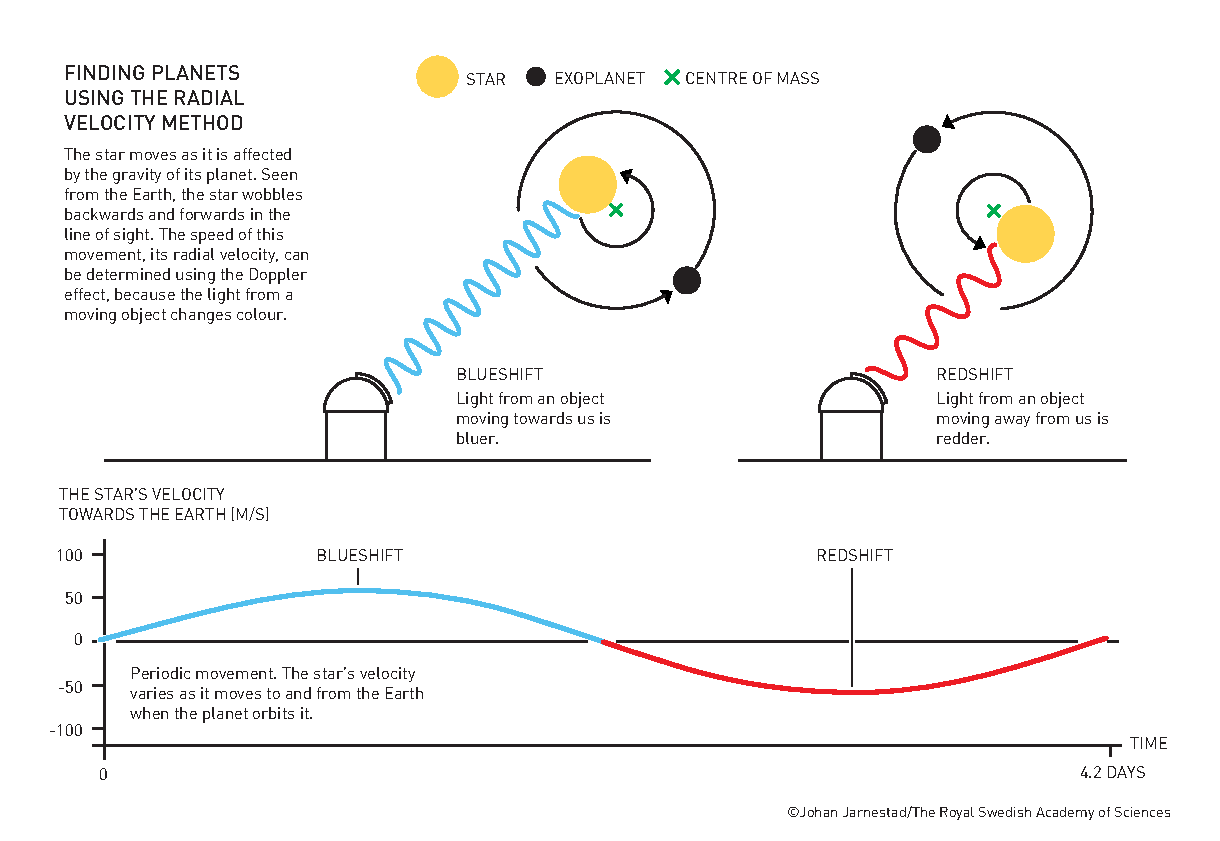
\includegraphics[width=\textwidth]{figures/rv_method_illustration.pdf}
        \caption{Illustration of the radial velocity method for exoplanet detection. © Johan Jarnestad/The Royal Swedish Academy of Sciences}
        \label{fig:rv_method_illustration}
    \end{wide}
\end{SCfigure}

A large planet like Jupiter induces a radial velocity (RV) in the Sun of about 12.7 m/s when observed in its plane of orbit. While a small one like Earth only induces an RV of about 9 cm/s. (p. 29, \cite{radial_velocity_techniques}). 

\vspace{0.5cm}
\todo{Possibly describe the RV calculation in more \href{http://exoplanets.astro.yale.edu/workshop/EPRV/Bibliography_files/Radial_Velocity.pdf}{detail} and compute Earth K. } 


\subsubsection{Doppler shift}

The radial velocity method relies on the well-known Doppler effect. Ignoring terms of $c^-4$ and higher, the general shift caused by a relative displacement betweeen the source and an observer at zero gravitatonal potential is given by 

\begin{equation}
    \label{eq:doppler_GR_SR}
    \lambda=\lambda_{0} \frac{1+\frac{1}{c} \mathbf{k} \cdot \mathbf{v}}{1-\frac{\Phi}{c^{2}}-\frac{v^{2}}{2 c^{2}}},
\end{equation}

which accounts for both special relativistic effects and gravitatonal doppler shift described by general relativity. Where $\lambda$ is the observed wavelength, $\lambda_0$ is the emitted wavelength, $\Phi$ is the Newtonian gravitational potential at the source $(\Phi=G M / r$ at a distance $r$ of a spherically symmetric mass $M$ ), $\textbf{k}$ is the unit vector pointing from the observer to the source, $\textbf{v}$ is the velocity of the source relative to the observer and $c$ is the speed of light \cite{doppler_shift_GR_formula}.

Special relativistic effects we can safely ignore, as we are dealing with velocity shifts on the order of meters or centimeters per second, and thereby cross out the third term in the denominator. The remaining terms $(1-\Phi/c^2)$ evaluted for HD 34411 ($M = (1.08 \pm 0.14) M_{\odot}$, $R = (1.28 \pm 0.04) R_{\odot}$ \cite{star_properties}) is around $0.999998$. Adding this term to the computation of RV does not change my results, so we can neglect the denominator completely. \todo{How to check analytically though?}

If the unit vector $\textbf{k}$ were pointing directly toward us, it would mean that we were observing the system in the plane of orbit. This is however unlikely. Since we don't know the inclication angle, a possible simplification is to omit $\textbf{k}$ is treat the resulting $\textbf{v}$ as a minimum radial velocity.

Thus we are left with 

\begin{equation}
    \label{eq:our_doppler}
    \lambda = \lambda_0 \times \Big(1 + \frac{v}{c} \Big),
\end{equation}

which is to say that the observed wavelength is simply the emitted wavelength scaled by a factor $(1 + v/c)$. This formula allows us to compute the minimum relative velocity shift, $v$, between two observations, $\lambda$ and $\lambda_0$.


\subsection{Description of the instrument}
The EXtreme PREcision Spectrograph or EXPRES is an extreme-precision spectrograph situated at the Lowell Observatory's 4.3m Lowell Discovery Telescope (LDT) near Flagstaff, Arizona, USA. The LDT allows for up to 280 partial nights of observation per year.

Like in many spectrographs, at the heart of EXPRES is a Charge Coupled Device (CCD). A CCD is a silicon-based multi-channel photon detector consisting of a large number of small light-sensitive areas called pixels. The CCD is EXPRES an STA1600LN CCD backside illuminated image sensor with a $10,560 \times 10,560$ array containing 9µm$\times$9µm pixels, designed to with a wavelength range of 3800$-$7800Å. When a photon hits a pixel it is converted into a charge, and each pixel can thus supply independent measurements. Since a one dimensional sensor would be impractical, EXPRES is constructed in such a way, that it wrap the spectrum inside the CDD, meaning that the spectrum starts in the top row of the sensor, and continues in the second row. Short wavelengths are thus to be found in the top of the CCD and long wavelengths at the bottom.
EXPRES is housed in a vacuum enclosure to minimize changes in temperature and pressure, which can otherwise cause the spectra to change position on the CCD and thus lead to errors in the RV mesaurements. 

\bigbreak
\noindent\textbf{Calibration device:}
Wavelength calibrations are performed with the use of a Laser Frequency Comb 
(LFC), produced by Menlo Systems, which is a laser source whose spectrum consists of a series of discrete, equally spaced frequency lines. The LFC however also needs calibration for which a Thorium Argon (ThAr) lamp with known frequencies is used.

\bigbreak
\noindent\textbf{Spectral resolution:}
EXPRES has a spectral resolution of $R = 150'000$, where R is defined as $R = \lambda / \Delta\lambda$. Inverting this we get what's called the resolution element of the instrumental spread Function (or line spread function), $\Delta\lambda = \lambda/R$. For a wavelength of say of $\lambda = 5000$Å, this comes out to $\Delta\lambda = 5000\text{Å}/150,000 \approx 0.033 $Å, and it describes the "blurring" of monochromatic beams on the detector. Absorption features narrower than $\Delta\lambda$ can, in a well-behaved spectrograph, be approximated as a normalized, symmetric Gausssian function with $\text{FWHM} = \Delta\lambda$. Specifically for EXPRES, a super-gauss is however a better fit\cite{yale_data}. LFC lines being monochromatic and thus very narrow will appear on the detector as a super-gaussian with $\Delta\lambda$ ranging from 3.9-5 pixels across the detector. By fitting, the center of the peak can be identified to a fraction of a pixel. The LFC lines are seperated by about 10 pixels to remain distinct after this blurring. For star-spectra however some emission and absorption lines will be too close together and will appear "blended" on the detector. 

\bigbreak
\noindent\textbf{Barycentric correction:}
Barycentric corrections are derived from the EXPRES exposure-meter, which is essentially a smaller, less precise spectrograph. Described in detail in \cite{barycentric_exposure_meter_blackman}. EXPRES as a whole is described in technical detail in \cite{EXPRES_technical_details_Jurgenson}.


\subsection{Description of the data}
EXPRES data are meant to serve as an example of the data being produced by next-generation spectrographs. 

The data used in this project was supplied by Lily Zhao and is by no means raw data, but data that has already gone through a lot of processing.

For development of RV extraction method, observations from four stars were used: 

\begin{itemize}
    \item HD 101501 (45 observations, 22 nights, Feb. 10, 2019 - Nov. 26, 2020)
    \item HD 26965 (114 observations, 37 nights, Aug. 20, 2019 - Nov. 27, 2020)
    \item HD 10700 (174 observations, 34 nights, Aug. 15, 2019 - Nov. 27, 2020)
    \item HD 34411 (188 observations, 58 nights, Oct. 08, 2019 - Nov. 27, 2020)
\end{itemize}

Most days have 3-4 observations, and there are significant gaps in the data as well. LFC exposure files were provided by Lars A. Buchhave. 

\subsubsection{Data structure}
The data used in this project consists of already packaged FITS (Flexible Image Transport System) files, which is a portable file standard widely used in the astronomy community to store images and tables. There is a FITS file for each observation, containing a variety of mesaurements for each pixel on the CCD. 
The rows of the CCD data are referred to as orders. There are 86 orders each of which has values from 7920 pixels. Drawing a coordinate system on the CCD, we are thus moving through pixels as we go along the x-axis and through orders as we go along the y-axis.

This would give the CCD the very elonganted dimensions of 86$\times$7920, but as mentioned earlier, the CCD is actually square. The orders however hit the CCD at an angle and for this reason \emph{order tracing} is necessary. Order tracing reduces each order from 2d array to a 1d array, which means the final image comes out much shorter in the vertical/order dimension. Described in detail in section 3.2.1 of \cite{first_RV_from_EXPRES}.

Furthermore, the CCD is not equally sensitive everywhere, and there are areas along the edges that are deemed useless. The data comes with a mask which shows which pixels are should be used. 

\subsubsection{Noise and corrections}
Photon noise and read noise are the two largest contributors to the noise on a given pixel on the EXPRES CCD. These two quantities are measured and summed in quadrature for each pixel. Photon noise is assumed to be poisson distributed and the standard deviation is then the square root of photon counts. Read noise is calculated emperically and is assumed to be consistent throughout each night of observation. \cite{first_RV_from_EXPRES}. 

Although manufactures have tried their best to limit it, the CCD still gets hits by scattering light, being the strongest in the center of the detector. This has been modeled and subtracted from the spectrum by measureing the photon count in between orders. The blaze function is available in the data file and allows for recovering the original counts for each pixel by multiplying the blaze with the spectrum.

Tellurics in the context of spectrographs refers to the contamination that ground based spectrographs must cope with, which occurs as the light passes through our atmosphere encountering molecules such as oxygen and water vapor on the way. The I use is already corrected for this, with a technique called SELENITE\cite{yale_data}.

The barycentric correction is vital, as this is what removes the movement of the Earth around the center-of-mass of the solar system from the data. How it is done exactly I've done delved into during this project. 

At the end, the largest source of error comes from stellar activity. Variations in the light from the star in quesiton due to various physical processes. Dark spots, granulation, "starquakes", rotation are a few examples. 

 

\section{Data Analysis}
\subsection{Calibration} 

    The calibration is needed to map each pixel on the CCD to a specific wavelength. Such a map is refered to as a wavelength solution. To do this, we need a light source with known frequencies, preferably many discret peaks. EXPRES uses a Thorium Argon lamp for an initial trial wavelength solution and a laser frequency comb (LFC) for an more precise solution.
    
    The Thorium Argon lamp produces 4,000 lines across 82 orders, which can be identified and mapped to a wavelength through a \emph{line atlas}. An intial wavelength solution for all pixels is then produced by linear interpolation. (I this project I have not done this calibration).

    The LFC generates a series of equadistant (evenly spaced) spectral lines, typically 20,000 lines across 50 orders. The range of the LFC is thus shorter, and for this reason the ThAr exposures can also be used for a rough calibration outside the LFC range. The frequencies of the LFC peaks are given by the relation
    
    \begin{equation}
        \label{eq:LFC_freq_eq}
        v_{n}=v_{\text{rep}} \times n+v_{\text{offset}}
    \end{equation}

    for integers $n$. The repetition rate $v_{\text {rep }}$ and offset frequency $v_{\text {offset }}$ are referenced against a GPS-disciplined quartz oscillator, providing calibration stability corresponding to a fractional uncertainty of less than $8 \times 10^{-12}$ for integration times greater than $1 \mathrm{~s}$. (p. 8, \cite{first_RV_from_EXPRES}). The values I have used in the calibration, $v_{\text{rep}} = 14e9$ and $v_{\text{offset}} = 6.19e9$, were provided by Lars Buchhave, but may be outdated. 

    The location of the LFC peaks (also refered to as modes) I determine first with a peak finding algorithm from scipy and then by fitting a super-gauss with a linear background to each peak:
    
    \begin{equation}
        \label{eq:LFC_super_gauss}
        A \exp \left(-\left(\frac{\left(x-\mu\right)^{2}}{2 \sigma_{x}^{2}}\right)^{P}\right) + B(x-\mu) + C
    \end{equation}
    
    A super-gauss is a regular gaussian but with an extra parameter, here denoted $P$, that allows the top of the peak to be flattened. To map the LFC peaks with the frequencies given by equation (\ref{eq:LFC_freq_eq})

    I can then use the intial wavelength solution (provided in the data that I have used) to map the LFC peaks to the frequencies given by equation (\ref{eq:LFC_freq_eq}). 

    From here, I have explored two approaches to produce a wavelength solution for all pixels: cubic interpolation and polynomial fit. I can evaluate the quality of the interpolation calibration by choosing to omit every second peak from the interpolation and then computing the residuals between the omitted peaks and the resulting interpolation function. For the polynomial, I can compute residuals simply by subtracting the location peaks from the fit function. Residuals from the two methods are compared in figure \ref{fig:calib_poly_vs_interp}.

    \begin{figure}[ht]
        \centering
        \includegraphics[scale=0.40]{figures/hist_peak_residuals_poly_and_interp3.png}
        \caption{Residuals from calibrations performed through poly-fit and interpolation. Both results contain approximately the same amount of points, but the poly-fit has a much larger spread and therefore appears smaller. \todo{polyfit has 18373 lines, interp has 16888. Why? } \todo{find out x units}}
        \label{fig:calib_poly_vs_interp}
    \end{figure}

    The standard deviation of the residuals from the interpolation come out much smaller than that of the polyfit (values specified in figure \ref{fig:calib_poly_vs_interp}), in this example, suggesting that the interpolation method is superior. It is also worth noting that because the interpolation was done on only half the data points, it will be even better when performed on all data points. A similar comparison was done to determine that the polynomial fit got better with increasing degrees until 5th. \todo{specify what file?}

    \vspace{0.5cm}

    \todo{add graph comparing residuals using gauss vs super gauss}

    \todo{perhaps add plot of changes in parameters across the CCD}

    \todo{specify run times for calibration using poly fit and interp}

\subsection{RV extraction}
    \begin{itemize}
        \item Hist fit / cross-correlation
        \begin{itemize}
            \item Order approach
            \item Feature approach
            \item (Run times)
        \end{itemize}
        \item Extracting relative radial velocities from over constraint system (Matrix reduction to circumvent correlations)
        \item Future ideas
        \begin{itemize}
            \item Auto encoder
        \end{itemize}
    \end{itemize}
 

\section{(Results)}
% 
In figure \ref*{fig:shift_matrix_barycentric} is plotted the $\Delta V_r^{ij}$ matrix for barycentric-corrected excalibur calibrated data for HD 34411. We are now on the order of m/s instead of km/s.

\begin{SCfigure}[1][!ht]%
    \begin{wide}  
        \includegraphics[width=\textwidth]{figures/shfits_matrix_bary.pdf}
        \caption{RV shifts matrix computed for HD34411 using excalibur calibrated, barycentric-corrected data (column \texttt{bary\char`_excalibur}). Each cell shows the median relative radial velocity across all features found between observations $i$ and $j$. The diagonal should be zero and has been ommited for the sake of computational speed.}
        \label{fig:shift_matrix_barycentric}
    \end{wide}
\end{SCfigure}

Performing the matrix reduction chi2 fit yields the results plotted in figure 

\begin{SCfigure}[1][!ht]%
    \begin{wide}  
        \includegraphics[width=\textwidth]{figures/HD34411_barycentric_rv_vs_lily.pdf}
        \caption{Computed relative wavelength shifts for HD34411 using excalibur calibrated, barycentric-corrected data (column \texttt{bary\char`_excalibur}). Top: my results \todo{Errors are too small}. Bottom: Lily Zhao's results using a chunk-by-chunk analysis. \todo{Cite?}}
        \label{fig:RV_results_barycentric}
    \end{wide}
\end{SCfigure}
 

\section{Discusion}
% \textbf{Future ideas:}
\begin{itemize}
    \item Errors
    \item Errors from the interpolation, the more points we sample the smaller the error??
    \item Filters: chauvenet's, rv cut, z-score cut
\end{itemize}


\textbf{Future ideas:}
\begin{itemize}
    \item Auto encoder
    \item Lunch LFC into orbit around earth to have a base truth
    \item Better understand the stellar activities
\end{itemize} 

\section{Conclusion}
% \input{sections/conclusion} 

%%%%%%%%%%%%%%%% Bibliography %%%%%%%%%%%%%%%%%%%%%%%%%%%%%%%%%%%%%%%%%%%%%%%
\newpage
\nocite{*}
\bibliographystyle{plain}
\bibliography{references.bib}

\end{document}
